\clearpage

\renewcommand{\thesection}{S\arabic{section}}
\renewcommand{\thetable}{S\arabic{table}}
\renewcommand{\thefigure}{S\arabic{figure}}
\renewcommand{\theequation}{S\arabic{equation}}
\setcounter{section}{0}
\setcounter{table}{0}
\setcounter{figure}{0}
\setcounter{equation}{0}

\section*{Supplementary Material: Can Aesthetic Emotions Explain Individual Taste? \\Investigating an Interpretable Route to Personalized Image Aesthetics}

This supplementary document provides complete experimental protocols, full statistical audits under Holm--Bonferroni correction, extended architecture and regularizer ablations, and detailed diagnostic tables supporting the main manuscript.

\section{Experimental and Statistical Details}
\label{sec:supp_exp_stat}
% -----------dataset detail----------------------
\subsection{Dataset Breakdown and First-Session Filtering}
The XPASS-Vis dataset~\cite{hayashi2026xpassvis} comprises 6,526 stimulus images and 87,836 individual rating interactions across 129 participants. \cref{tab:domain_counts} breaks down these interactions across the three evaluated visual domains. 

\begin{table}[h]
\centering
\caption{XPASS-Vis images and rating interactions per domain.}
\label{tab:domain_counts}
\begin{tabular}{lrr}
\toprule
Domain & Images & Interactions \\
\midrule
Artwork    & 2{,}345 & 31{,}543 \\
Fashion    & 2{,}082 & 28{,}154 \\
Landscape  & 2{,}099 & 28{,}139 \\
\midrule
Total      & 6{,}526 & 87{,}836 \\
\bottomrule
\end{tabular}
\end{table}

% -------------------------------------------------
% Table S2: Backbone
\begin{table*}[t]
\centering
\footnotesize
\setlength{\tabcolsep}{4.5pt}
\caption{Performance comparison of Population (Ridge), Direct (Ridge) and Hybrid (Ridge) across visual backbones and image domains (mean $\pm$ SEM over user--domain units).}
\label{tab:backbone}
\begin{threeparttable}
    \begin{tabular}{ll cc cc cc cc}
\toprule
\multirow{2}{*}{Backbone} & \multirow{2}{*}{Model} & \multicolumn{2}{c}{Artwork} & \multicolumn{2}{c}{Fashion} & \multicolumn{2}{c}{Landscape} & \multicolumn{2}{c}{Average} \\
\cmidrule(lr){3-4}\cmidrule(lr){5-6}\cmidrule(lr){7-8}\cmidrule(lr){9-10}
 & & SROCC & PLCC & SROCC & PLCC & SROCC & PLCC & SROCC & PLCC \\
\midrule
\multirow{3}{*}{CLIP frozen} & Population & $.465_{\pm .017}$ & $.474_{\pm .016}$ & $.326_{\pm .013}$ & $.347_{\pm .013}$ & $.457_{\pm .015}$ & $.459_{\pm .014}$ & $.416_{\pm .011}$ & $.427_{\pm .011}$ \\
& Direct & $\bm{.524_{\pm .014}}$ & $\bm{.533_{\pm .014}}$ & $\bm{.365_{\pm .013}}$ & $\bm{.382_{\pm .013}}$ & $.478_{\pm .015}$ & $\bm{.489_{\pm .014}}$ & $\bm{.456_{\pm .011}}$ & $\bm{.468_{\pm .010}}$ \\
& Hybrid & $.486_{\pm .017}^{\dagger}$ & $.493_{\pm .016}^{\dagger}$ & $.338_{\pm .014}$ & $.356_{\pm .013}^{\dagger}$ & $\bm{.481_{\pm .014}}^{\dagger}$ & $.486_{\pm .014}^{\dagger}$ & $.435_{\pm .011}^{\dagger}$ & $.445_{\pm .011}^{\dagger}$ \\
\addlinespace
\multirow{3}{*}{CLIP-ft (score)} & Population & $.470_{\pm .017}$ & $.477_{\pm .016}$ & $.332_{\pm .013}$ & $.347_{\pm .013}$ & $.452_{\pm .014}$ & $.455_{\pm .014}$ & $.418_{\pm .011}$ & $.426_{\pm .010}$ \\
& Direct & $\bm{.539_{\pm .013}}$ & $\bm{.542_{\pm .013}}$ & $\bm{.355_{\pm .013}}$ & $\bm{.375_{\pm .013}}$ & $\bm{.482_{\pm .015}}$ & $\bm{.487_{\pm .014}}$ & $\bm{.459_{\pm .010}}$ & $\bm{.468_{\pm .010}}$ \\
& Hybrid & $.488_{\pm .016}^{\dagger}$ & $.493_{\pm .016}$ & $.340_{\pm .013}$ & $.353_{\pm .013}$ & $.472_{\pm .014}^{\dagger}$ & $.477_{\pm .014}^{\dagger}$ & $.434_{\pm .011}^{\dagger}$ & $.441_{\pm .010}^{\dagger}$ \\
\addlinespace
\multirow{3}{*}{CLIP-ft (emotion)} & Population & $.468_{\pm .016}$ & $.473_{\pm .016}$ & $.315_{\pm .014}$ & $.329_{\pm .013}$ & $.435_{\pm .015}$ & $.438_{\pm .014}$ & $.406_{\pm .011}$ & $.413_{\pm .010}$ \\
& Direct & $\bm{.525_{\pm .013}}$ & $\bm{.531_{\pm .013}}$ & $\bm{.349_{\pm .015}}$ & $\bm{.362_{\pm .014}}$ & $\bm{.473_{\pm .015}}$ & $\bm{.479_{\pm .015}}$ & $\bm{.449_{\pm .011}}$ & $\bm{.457_{\pm .011}}$ \\
& Hybrid & $.486_{\pm .015}^{\dagger}$ & $.492_{\pm .015}^{\dagger}$ & $.328_{\pm .015}$ & $.341_{\pm .015}$ & $.456_{\pm .015}^{\dagger}$ & $.463_{\pm .015}^{\dagger}$ & $.423_{\pm .011}^{\dagger}$ & $.432_{\pm .011}^{\dagger}$ \\
\addlinespace
\multirow{3}{*}{Qwen3-VL 4B} & Population & $.476_{\pm .017}$ & $.486_{\pm .016}$ & $.363_{\pm .013}$ & $.374_{\pm .013}$ & $.469_{\pm .014}$ & $.472_{\pm .014}$ & $.436_{\pm .011}$ & $.444_{\pm .011}$ \\
& Direct & $\bm{.532_{\pm .013}}$ & $\bm{.539_{\pm .013}}$ & $\bm{.382_{\pm .014}}$ & $\bm{.394_{\pm .013}}$ & $\bm{.496_{\pm .014}}$ & $\bm{.501_{\pm .014}}$ & $\bm{.470_{\pm .011}}$ & $\bm{.478_{\pm .010}}$ \\
& Hybrid & $.488_{\pm .016}$ & $.495_{\pm .016}$ & $.365_{\pm .015}$ & $.377_{\pm .014}$ & $.492_{\pm .014}^{\dagger}$ & $.499_{\pm .014}^{\dagger}$ & $.448_{\pm .012}^{\dagger}$ & $.457_{\pm .011}^{\dagger}$ \\
\addlinespace
\multirow{3}{*}{Qwen3-VL 8B} & Population & $.477_{\pm .017}$ & $.487_{\pm .017}$ & $.372_{\pm .013}$ & $.384_{\pm .013}$ & $.469_{\pm .015}$ & $.475_{\pm .014}$ & $.439_{\pm .011}$ & $.449_{\pm .011}$ \\
& Direct & $\bm{.534_{\pm .014}}$ & $\bm{.542_{\pm .014}}$ & $\bm{.398_{\pm .013}}$ & $\bm{.412_{\pm .013}}$ & $\bm{.501_{\pm .015}}$ & $\bm{.510_{\pm .015}}$ & $\bm{.478_{\pm .011}}$ & $\bm{.488_{\pm .010}}$ \\
& Hybrid & $.496_{\pm .016}^{\dagger}$ & $.504_{\pm .016}$ & $.386_{\pm .014}$ & $.398_{\pm .013}^{\dagger}$ & $.496_{\pm .015}^{\dagger}$ & $.504_{\pm .015}^{\dagger}$ & $.459_{\pm .011}^{\dagger}$ & $.469_{\pm .011}^{\dagger}$ \\
\bottomrule
\end{tabular}

    \begin{tablenotes}[flushleft]\footnotesize
    \item Domain columns are over $n=129$ paired participants; the Average column uses a participant-cluster bootstrap over 129 participants.
    \item $\dagger$ indicates that Hybrid significantly outperforms Population after Holm correction within the corresponding backbone--domain--metric family. Direct is reported descriptively and is not included in these tests. The superior predictive model is in \textbf{bold}.
    \end{tablenotes}
\end{threeparttable}
\end{table*}

% --------------------------------------------------
% reproducibility
\textbf{Reproducibility.}
To eliminate non-deterministic thread-scheduling noise in multi-threaded BLAS operations, matrix operations are pinned to a single thread for the whole run, set before NumPy is imported. Candidates whose validation SROCC differs by less than $10^{-9}$ are treated as tied and resolved via an explicit tie-breaking rule favoring the stronger regularization penalty. All random projections, permutations and initializations are tied to fixed, per-fold seeds. Results are averaged over three run-level seeds.
Experiments were run with Python 3.11, NumPy 1.26, scikit-learn 1.4, SciPy 1.11 and PyTorch 2.2. Code, split files and the scripts that regenerate every table and figure are available at \url{https://anonymous.4open.science/r/piaa-emotion-mediated-anonymous-DF01/}.
% ---------------------------------------------------

\subsection{Joint Concept Bottleneck Formulation}
\label{sec:supp_joint}
%  --------MLP -----------
To evaluate whether linearity imposes a performance ceiling, we compare it against two non-linear alternatives where both stages use single-hidden-layer MLPs:
\begin{enumerate}[noitemsep,topsep=2pt]
    \item \emph{MLP $\to$ MLP (Sequential):} A shared MLP $h$ is trained on emotion targets and frozen; a personal MLP $g_u$ is then trained on its output.
    \item \emph{MLP $\to$ MLP (Joint):} A shared MLP $h$ is trained simultaneously on emotion targets and the population aesthetic score, with the score read directly from the seven bottleneck concepts so that task gradients flow through the semantic layer. The personal head $g_u$ is then trained on the frozen bottleneck outputs.
\end{enumerate}
% ---
Joint training is strictly confined to the shared population stage; it is not extended end-to-end into individual personal heads. Fine-tuning $h$ per user would require estimating hundreds of thousands of parameters from only $\sim$100 samples per user, which would induce severe overfitting and eliminate the parameter efficiency of our method.
The joint extractor optimizes an equally weighted objective ($L = \frac{1}{2}\text{MSE}_{\text{score}} + \frac{1}{2}\lambda\text{MSE}_{\text{emotion}}$) where $\text{MSE}_{\text{emotion}}$ is averaged over the seven concepts. The aesthetic head branches directly from the 7-dimensional emotion layer, forcing score gradients through the semantic bottleneck.

\textbf{Hyperparameter Selection and Training Protocols.}
Each head has a single hyperparameter selected by mirroring the test protocol on the validation group: the ridge penalty $\alpha$ is tuned over a 17-value logarithmic grid ($10^{-6}$ to $10^{10}$), and the MLP learning rate over an 11-value logarithmic grid from $10^{-4}$ to $10$. Both are chosen on validation-group users, then frozen before any test user is fitted. 
MLP training uses mean squared error loss, with no weight decay, and every MLP is trained for a fixed 500 epochs with Adam optimizer. Early stopping with an internal validation split was omitted because, with support sets as small as 10 ratings, an 85/15 split leaves only 1--2 samples, providing an unstable stopping signal.

% ---------------MLP baseline---------------
\begin{table}[t]
    \centering
    \begin{tabular}{ll cc cc cc cc}
\toprule
\multirow{2}{*}{Mediator} & \multirow{2}{*}{Head} & \multicolumn{2}{c}{Artwork} & \multicolumn{2}{c}{Fashion} & \multicolumn{2}{c}{Landscape} & \multicolumn{2}{c}{Average} \\
\cmidrule(lr){3-4}\cmidrule(lr){5-6}\cmidrule(lr){7-8}\cmidrule(lr){9-10}
& & SROCC & PLCC & SROCC & PLCC & SROCC & PLCC & SROCC & PLCC \\
\midrule
\multirow{2}{*}{Population} & Ridge & $.477_{\pm .017}$ & $.487_{\pm .017}$ & $.372_{\pm .013}$ & $.384_{\pm .013}$ & $.469_{\pm .015}$ & $.475_{\pm .014}$ & $.439_{\pm .011}$ & $.449_{\pm .011}$ \\
 & MLP & $.427_{\pm .016}$ & $.438_{\pm .016}$ & $.303_{\pm .011}$ & $.316_{\pm .012}$ & $.401_{\pm .013}$ & $.406_{\pm .013}$ & $.377_{\pm .010}$ & $.386_{\pm .010}$ \\
\addlinespace
\multirow{2}{*}{Direct} & Ridge & $.534_{\pm .014}$ & $.542_{\pm .014}$ & $.398_{\pm .013}$ & $.412_{\pm .013}$ & $.501_{\pm .015}$ & $.510_{\pm .015}$ & $.478_{\pm .011}$ & $.488_{\pm .010}$ \\
 & MLP & $.356_{\pm .014}$ & $.354_{\pm .014}$ & $.234_{\pm .012}$ & $.238_{\pm .012}$ & $.336_{\pm .015}$ & $.339_{\pm .015}$ & $.309_{\pm .010}$ & $.310_{\pm .010}$ \\
\addlinespace
\multirow{2}{*}{Random} & Ridge & $.495_{\pm .015}$ & $.504_{\pm .015}$ & $.373_{\pm .013}$ & $.384_{\pm .012}$ & $.473_{\pm .014}$ & $.480_{\pm .014}$ & $.447_{\pm .010}$ & $.456_{\pm .010}$ \\
 & MLP & $.479_{\pm .013}$ & $.484_{\pm .014}$ & $.328_{\pm .012}$ & $.339_{\pm .012}$ & $.431_{\pm .014}$ & $.431_{\pm .014}$ & $.412_{\pm .010}$ & $.418_{\pm .010}$ \\
\addlinespace
\multirow{2}{*}{PCA} & Ridge & $.510_{\pm .015}$ & $.519_{\pm .015}$ & $.377_{\pm .014}$ & $.388_{\pm .013}$ & $.487_{\pm .015}$ & $.495_{\pm .015}$ & $.458_{\pm .011}$ & $.467_{\pm .011}$ \\
 & MLP & $.495_{\pm .015}$ & $.504_{\pm .015}$ & $.350_{\pm .013}$ & $.359_{\pm .013}$ & $.466_{\pm .016}$ & $.469_{\pm .016}$ & $.437_{\pm .011}$ & $.444_{\pm .011}$ \\
\addlinespace
\multirow{2}{*}{Hybrid (ours)} & Ridge & $.496_{\pm .016}$ & $.504_{\pm .016}$ & $.386_{\pm .014}$ & $.398_{\pm .013}$ & $.496_{\pm .015}$ & $.504_{\pm .015}$ & $.459_{\pm .011}$ & $.469_{\pm .011}$ \\
 & MLP & $.459_{\pm .015}$ & $.468_{\pm .016}$ & $.315_{\pm .013}$ & $.325_{\pm .012}$ & $.437_{\pm .015}$ & $.441_{\pm .014}$ & $.404_{\pm .011}$ & $.411_{\pm .010}$ \\
\bottomrule
\end{tabular}

% Descriptive table: no significance markers.
% Qwen3-VL 8B, population-anchored, N=100; seeds averaged within units.

    \caption{\textbf{Sequential MLP architectures for the emotion mediator and personal head.} Evaluated on CLIP frozen, unanchored, $N=100$.}
    \label{tab:mlp_baseline}
\end{table}

\begin{table*}[t]
\centering
\begin{threeparttable}
    \caption{\textbf{Head and training scheme for the emotion mediator, and the weight on the joint concept loss.} Qwen3-VL 8B, population-anchored, $N=100$, averaged over user--domain units and three seeds. The joint rows train the two shared stages together on $\mathcal{L} = \mathrm{MSE}(\hat{y}) + \lambda\,\mathrm{MSE}(\hat{c})$, which is the joint concept-bottleneck objective of Koh et al.~\cite{koh2020cbm} with unit weight on the task loss ($\lambda$).}
\label{tab:mlp}
\small
\setlength{\tabcolsep}{4pt}
\begin{tabular}{@{}l cc cc cc cc@{}}
\toprule
\multirow{2}{*}{Stage-1 $\to$ Stage-2} & \multicolumn{2}{c}{Artwork} & \multicolumn{2}{c}{Fashion} & \multicolumn{2}{c}{Landscape} & \multicolumn{2}{c}{Average} \\
\cmidrule(lr){2-3}\cmidrule(lr){4-5}\cmidrule(lr){6-7}\cmidrule(lr){8-9}
& SROCC & PLCC & SROCC & PLCC & SROCC & PLCC & SROCC & PLCC \\
\midrule
Ridge $\to$ Ridge (main) & $\bm{.496_{\pm .016}}$ & $\bm{.504_{\pm .016}}$ & $\bm{.386_{\pm .014}}$ & $\bm{.398_{\pm .013}}$ & $\bm{.496_{\pm .015}}$ & $\bm{.504_{\pm .015}}$ & $\bm{.459_{\pm .011}}$ & $\bm{.469_{\pm .011}}$ \\
\addlinespace
MLP $\to$ MLP, joint $\lambda=0.1$ & $.430_{\pm .016}$ & $.437_{\pm .016}$ & $.278_{\pm .012}$ & $.289_{\pm .012}$ & $.392_{\pm .015}$ & $.395_{\pm .015}$ & $.367_{\pm .010}$ & $.374_{\pm .010}$ \\
MLP $\to$ MLP, joint $\lambda=1$ & $.450_{\pm .015}$ & $.456_{\pm .016}$ & $.301_{\pm .012}$ & $.315_{\pm .012}$ & $.413_{\pm .015}$ & $.415_{\pm .014}$ & $.388_{\pm .011}$ & $.395_{\pm .010}$ \\
MLP $\to$ MLP, joint $\lambda=10$ & $.460_{\pm .015}$ & $.467_{\pm .015}$ & $.310_{\pm .013}$ & $.323_{\pm .012}$ & $.436_{\pm .015}$ & $.439_{\pm .014}$ & $.402_{\pm .011}$ & $.410_{\pm .011}$ \\
\addlinespace
MLP $\to$ MLP, sequential & $.459_{\pm .015}$ & $.468_{\pm .016}$ & $.315_{\pm .013}$ & $.325_{\pm .012}$ & $.437_{\pm .015}$ & $.441_{\pm .014}$ & $.404_{\pm .011}$ & $.411_{\pm .010}$ \\
\bottomrule
\end{tabular}

% Descriptive table: no significance markers.
% Average SEM uses a 129-participant cluster bootstrap.

\begin{tablenotes}[flushleft]\footnotesize
    \item Values are mean $\pm$ 1 SEM over 387 user--domain units ($n=129$ per domain; the Average column uses a participant-cluster bootstrap). Best value per column in \textbf{bold}.
    \item Ridge $\to$ Ridge achieves the highest entry in every domain and on both metrics, so we use ridge heads throughout.
\end{tablenotes}
\end{threeparttable}
\end{table*}

\textbf{Every entry in this table is significantly below Ridge $\to$ Ridge}, in every domain and on both metrics, by paired Wilcoxon signed-rank test over the same 387 units.
 % ---------------linear rgressor ablation-------------
\begin{table}[t]
\centering
\begin{threeparttable}
\caption{\textbf{Choice of regulariser for the personal head.} CLIP frozen, no anchor, $N=100$, three seeds, 387 user--domain units.}
\label{tab:regulariser}
\small
\setlength{\tabcolsep}{4pt}
\begin{tabular}{@{}l cc cc cc@{}}
\toprule
\multirow{2}{*}{Head} & \multicolumn{2}{c}{Population} & \multicolumn{2}{c}{Direct} & \multicolumn{2}{c}{Hybrid (ours)} \\
\cmidrule(lr){2-3}\cmidrule(lr){4-5}\cmidrule(lr){6-7}
 & SROCC & PLCC & SROCC & PLCC & SROCC & PLCC \\
\midrule
Ridge       & $.416_{\pm .011}$ & $.427_{\pm .011}$ & $.400_{\pm .012}$ & $.410_{\pm .012}$ & $\bm{.419_{\pm .011}}$ & $\bm{.429_{\pm .011}}$ \\
Lasso       & $.412_{\pm .011}$ & $.422_{\pm .011}$ & $.330_{\pm .012}$ & $.340_{\pm .012}$ & $.418_{\pm .011}$ & $.428_{\pm .011}$ \\
Elastic net & $.412_{\pm .011}$ & $.422_{\pm .011}$ & $.344_{\pm .012}$ & $.354_{\pm .012}$ & $.419_{\pm .011}$ & $.428_{\pm .011}$ \\
\bottomrule
\end{tabular}
\begin{tablenotes}[flushleft]\footnotesize
\item Values are mean $\pm$ 1 SEM over user--domain units using a participant-cluster bootstrap.
\item The emotion bottleneck is insensitive to the choice of regulariser (.419, .418, .419), because seven standardised inputs leave little for a sparsity penalty to remove. The direct model is not: $\ell_1$ shrinkage drops it from .400 to .330, and the elastic net to .344, since discarding coordinates of a 512-dimensional embedding destroys information that no single coordinate carries alone.
\item We therefore use ridge throughout. This experiment predates the population anchor and is reported on the unanchored setting.
\end{tablenotes}
\end{threeparttable}
\end{table}
 % ----------------------------------------------------
% -----------distribution sd14dim, hist35dim
\begin{table}[t]
\centering
\begin{threeparttable}
    \caption{\textbf{Distribution-valued Stage-1 targets.} CLIP frozen, population-anchored, ridge head, three seeds, 387 user--domain units. Widths are 7 (per-emotion mean), 14 (mean and across-rater standard deviation) and 35 (7 emotions $\times$ 5 rating-histogram bins).}
    \label{tab:distribution}
    \small
    \setlength{\tabcolsep}{3.5pt}
        \begin{tabular}{@{}c cc ccc@{}}
        \toprule
        $N$ & Population & Direct & Hybrid 7-d & Hybrid 14-d & Hybrid 35-d \\
        \midrule
        10  & $.416$ & $.420$ & $.414$ & $.419$ & $.413$ \\
        25  & $.416$ & $.431$ & $.415$ & $.419$ & $.425$ \\
        50  & $.416$ & $.440$ & $.423$ & $.428$ & $.435$ \\
        100 & $.416$ & $.456$ & $.435$ & $.434$ & $.442$ \\
        \bottomrule
        \end{tabular}
    \begin{tablenotes}[flushleft]\footnotesize
    \item Values are mean SROCC over 387 user--domain units reported descriptively.
    \item The 14-d variant yields similar means to the 7-d mediator at $N=100$ (.434 against .435). The 35-d histogram performs slightly higher at $N\ge25$, but at five times the width of the bottleneck.
    \item This experiment was run on CLIP frozen only and is reported as a negative control for the choice of Stage-1 target, not as a primary result.
    \end{tablenotes}
\end{threeparttable}
\end{table}
 % ----------------------------------------------------
%  % RQ2.1 emotion accuracy
% \begin{table*}[t]
% \centering
% \begin{threeparttable}
% \caption{\textbf{Stage-1 emotion extraction accuracy.}}
% \label{tab:stage1_accuracy}
% \small
% \setlength{\tabcolsep}{4.5pt}
% \begin{tabular}{l cc cc cc cc}
\toprule
\multirow{2}{*}{Concept} & \multicolumn{2}{c}{Artwork} & \multicolumn{2}{c}{Fashion} & \multicolumn{2}{c}{Landscape} & \multicolumn{2}{c}{Average} \\
\cmidrule(lr){2-3}\cmidrule(lr){4-5}\cmidrule(lr){6-7}\cmidrule(lr){8-9}
 & SROCC & PLCC & SROCC & PLCC & SROCC & PLCC & SROCC & PLCC \\
\midrule
\textit{Amused} & $.684_{\pm .036}$ & $.696_{\pm .033}$ & $.450_{\pm .045}$ & $.463_{\pm .048}$ & $\bm{.687_{\pm .023}}$ & $\bm{.687_{\pm .023}}$ & $\bm{.607_{\pm .035}}$ & $.615_{\pm .035}$ \\
\textit{Distasteful} & $.682_{\pm .023}$ & $.686_{\pm .018}$ & $\bm{.562_{\pm .031}}$ & $\bm{.601_{\pm .028}}$ & $.569_{\pm .022}$ & $.583_{\pm .024}$ & $.604_{\pm .020}$ & $\bm{.623_{\pm .017}}$ \\
\textit{Impressed} & $\bm{.694_{\pm .029}}$ & $.704_{\pm .029}$ & $.449_{\pm .033}$ & $.472_{\pm .032}$ & $.649_{\pm .014}$ & $.665_{\pm .016}$ & $.597_{\pm .032}$ & $.614_{\pm .031}$ \\
\textit{Intellectual} & $.487_{\pm .052}$ & $.503_{\pm .053}$ & $.371_{\pm .041}$ & $.384_{\pm .047}$ & $.563_{\pm .039}$ & $.597_{\pm .031}$ & $.474_{\pm .032}$ & $.495_{\pm .033}$ \\
\textit{Motivated} & $.545_{\pm .039}$ & $.587_{\pm .044}$ & $.346_{\pm .048}$ & $.362_{\pm .044}$ & $.537_{\pm .033}$ & $.550_{\pm .035}$ & $.476_{\pm .033}$ & $.500_{\pm .034}$ \\
\textit{Nostalgic} & $.683_{\pm .022}$ & $\bm{.717_{\pm .026}}$ & $.378_{\pm .022}$ & $.395_{\pm .025}$ & $.617_{\pm .027}$ & $.673_{\pm .019}$ & $.559_{\pm .037}$ & $.595_{\pm .040}$ \\
\textit{Sad} & $.556_{\pm .036}$ & $.573_{\pm .036}$ & $.317_{\pm .029}$ & $.375_{\pm .023}$ & $.460_{\pm .037}$ & $.512_{\pm .028}$ & $.445_{\pm .032}$ & $.487_{\pm .027}$ \\
\bottomrule
\end{tabular}

% \end{threeparttable}
% \end{table*}
% ------------------------------------------------------
% efficientcy graph detail
% \begin{table*}[t]
% \centering
% \small
% \begin{threeparttable}
% \caption{\textbf{Efficiency and Mediator Comparison.} Personalization performance (SROCC and PLCC) across sample sizes $N$ with Qwen3-VL 8B (Population Anchored).}
% \label{tab:efficiency_full}
% \begin{tabular}{ll cc cc cc cc}
% \toprule
% \multirow{2}{*}{$N$} & \multirow{2}{*}{\textbf{Model}} 
%   & \multicolumn{2}{c}{\textbf{Artwork}} 
%   & \multicolumn{2}{c}{\textbf{Fashion}} 
%   & \multicolumn{2}{c}{\textbf{Landscape}} 
%   & \multicolumn{2}{c}{\textbf{Average}} \\
% \cmidrule(lr){3-4} \cmidrule(lr){5-6} \cmidrule(lr){7-8} \cmidrule(lr){9-10}
%   & & \textbf{SROCC} & \textbf{PLCC} 
%     & \textbf{SROCC} & \textbf{PLCC} 
%     & \textbf{SROCC} & \textbf{PLCC} 
%     & \textbf{SROCC} & \textbf{PLCC} \\
% \midrule
% \multicolumn{2}{l}{\textit{Population}} 
%   & $.477_{\pm .017}$ & $.487_{\pm .017}$ 
%   & $.372_{\pm .013}$ & $.384_{\pm .013}$ 
%   & $.469_{\pm .015}$ & $.475_{\pm .014}$ 
%   & $.439_{\pm .009}$ & $.449_{\pm .009}$ \\
% \addlinespace
% 10 & Direct & $.486_{\pm .016}$ & $.498_{\pm .016}$ & $.368_{\pm .013}$ & $.381_{\pm .012}$ & $.458_{\pm .015}$ & $.464_{\pm .015}$ & $.437_{\pm .009}$ & $.448_{\pm .009}$ \\
%    & Hybrid & $.481_{\pm .017}$ & $.490_{\pm .016}$ & $.347_{\pm .015}$ & $.360_{\pm .015}$ & $.472_{\pm .015}$ & $.479_{\pm .015}$ & $.433_{\pm .010}$ & $.443_{\pm .009}$ \\
% \addlinespace
% 25 & Direct & $.494_{\pm .016}$ & $.504_{\pm .016}$ & $.376_{\pm .013}$ & $.389_{\pm .013}$ & $.481_{\pm .014}$ & $.489_{\pm .014}$ & $.450_{\pm .009}$ & $.460_{\pm .009}$ \\
%    & Hybrid & $.478_{\pm .017}$ & $.487_{\pm .016}$ & $.368_{\pm .014}$ & $.380_{\pm .014}$ & $.478_{\pm .015}$ & $.486_{\pm .015}$ & $.442_{\pm .009}$ & $.451_{\pm .009}$ \\
% \addlinespace
% 50 & Direct & $.516_{\pm .014}$ & $.524_{\pm .014}$ & $.382_{\pm .013}$ & $.393_{\pm .012}$ & $.493_{\pm .014}$ & $.503_{\pm .014}$ & $.464_{\pm .009}$ & $.473_{\pm .008}$ \\
%    & Hybrid & $.488_{\pm .016}$ & $.496_{\pm .016}$ & $.374_{\pm .014}$ & $.383_{\pm .013}$ & $.489_{\pm .015}$ & $.499_{\pm .015}$ & $.450_{\pm .009}$ & $.459_{\pm .009}$ \\
% \addlinespace
% 100 & Direct & $.534_{\pm .014}$ & $.542_{\pm .014}$ & $.398_{\pm .013}$ & $.412_{\pm .013}$ & $.501_{\pm .015}$ & $.510_{\pm .015}$ & $.478_{\pm .009}$ & $.488_{\pm .008}$ \\
%     & Hybrid & $.496_{\pm .016}$ & $.504_{\pm .016}$ & $.386_{\pm .014}$ & $.398_{\pm .013}$ & $.496_{\pm .015}$ & $.504_{\pm .015}$ & $.459_{\pm .009}$ & $.469_{\pm .009}$ \\
% \bottomrule
% \end{tabular}
% \begin{tablenotes}[flushleft]\footnotesize
%     \item Values are $\text{Mean} \pm 1\text{ SEM}$ over user-domain units ($n=129$ per domain; the Average column pools each participant's three domains).
%     \item This table reports the numbers across rating budgets. Significance for the $N=100$ comparisons is given in \cref{tab:main}.
% \end{tablenotes}
% \end{threeparttable}
% \end{table*}
% --------------------------------
% faithful grapth detail
\begin{table}[t]
\centering
\small
\setlength{\tabcolsep}{6pt}
\renewcommand{\arraystretch}{0.95}
\begin{threeparttable}
\caption{\textbf{Formula Swap Evaluation.} Cross-user formula permutation test evaluating personalization specificity under Pop-Anchored and Unanchored (Plain) settings.}
\label{tab:formula_swap}
\begin{tabular}{ll cc}
\toprule
Setting & Formula & SROCC & PLCC \\
\midrule
\multirow{3}{*}{Anchored} 
& Own    & $\bm{.459_{\pm .012}}$ & $\bm{.469_{\pm .011}}$ \\
& Pop    & $.439_{\pm .011}^\downarrow$ & $.449_{\pm .011}^\downarrow$ \\
& Other  & $.396_{\pm .010}^\downarrow$ & $.403_{\pm .010}^\downarrow$ \\
\addlinespace
\multirow{3}{*}{Unanchored} 
& Own    & $.446_{\pm .011}$ & $.454_{\pm .010}$  \\
& Pop    & $.425_{\pm .011}^\downarrow$ & $.434_{\pm .011}^\downarrow$ \\
& Other  & $.368_{\pm .009}^\downarrow$ & $.376_{\pm .009}^\downarrow$ \\
\bottomrule
\end{tabular}
\begin{tablenotes}[flushleft]\footnotesize
    \item Values are mean $\pm$ 1 SEM over 387 user--domain units; SEM and tests use a participant-cluster bootstrap over 129 participants.
    \item $\downarrow$ marks a significant drop from the user's \emph{Own} formula, Holm-corrected within the setting (all Holm-adjusted $p<.001$).
\end{tablenotes}
\end{threeparttable}
\end{table}
% ----------------------------
\begin{table}[t]
\centering
\small
\setlength{\tabcolsep}{6pt}
\renewcommand{\arraystretch}{0.95}
\begin{threeparttable}
\caption{\textbf{Concept Ablation on Total Linear Weights.} Impact of holding individual emotion dimensions constant at support-set baselines.}
\label{tab:concept_ablation}
\begin{tabular}{l ccc}
\toprule
\textbf{Setting} & \textbf{SROCC} & \textbf{PLCC} & \textbf{SROCC Drop ($\Delta$)} \\
\midrule
Full         & $\bm{.459_{\pm .012}}$ & $\bm{.469_{\pm .011}}$ & --- \\
w/o Bottom   & $.459_{\pm .012}$ & $.468_{\pm .011}$ & $-0.0003$ \\
w/o Average  & $.435_{\pm .011}^\downarrow$ & $.444_{\pm .011}^\downarrow$ & $-0.0239$  \\
w/o Top      & $.361_{\pm .012}^\downarrow$ & $.367_{\pm .011}^\downarrow$ & $-0.0979$ \\
\bottomrule
\end{tabular}
\begin{tablenotes}[flushleft]\footnotesize
    \item Values are mean $\pm$ 1 SEM over user-domain units; SEM and tests use a participant-cluster bootstrap over 129 participants.
    \item $\downarrow$ marks a significant drop from the \emph{Full} model, Holm-corrected within the table (Top and Average $p<.001$; Bottom SROCC $p=.628$, PLCC $p=.036$).
\end{tablenotes}
\end{threeparttable}
\end{table}
% --------------------------------------------------
% image swap table detail
\begin{table}[t]
\centering
\small
\setlength{\tabcolsep}{6pt}
\renewcommand{\arraystretch}{0.95}
\begin{threeparttable}
\caption{\textbf{Image Swap Evaluation.} Cross-stimulus emotion permutation test evaluating image specificity under Pop-Anchored and Unanchored (Plain) settings.}
\label{tab:image_swap}
\begin{tabular}{ll cc}
\toprule
Setting & Emotion input & SROCC & PLCC \\
\midrule
\multirow{3}{*}{Anchored} 
& Correct image    & $\bm{.459_{\pm .012}}$ & $\bm{.469_{\pm .011}}$ \\
& Swapped image    & $.384_{\pm .010}^{\downarrow}$ & $.392_{\pm .010}^{\downarrow}$ \\
& No-image emotion & $.439_{\pm .011}^{\downarrow}$ & $.449_{\pm .011}^{\downarrow}$ \\
\addlinespace
\multirow{2}{*}{Unanchored} 
& Correct image    & $\bm{.446_{\pm .011}}$ & $\bm{.454_{\pm .010}}$ \\
& Swapped image    & $-.009_{\pm .000}^{\downarrow}$ & $-.009_{\pm .000}^{\downarrow}$ \\
\bottomrule
\end{tabular}
\begin{tablenotes}[flushleft]\footnotesize
    \item Values are mean $\pm$ 1 SEM over 387 user--domain units across all 49 non-zero cyclic image shifts; SEM and tests use a participant-cluster bootstrap over 129 participants.
    \item $\downarrow$ marks a significant drop from the \emph{Correct image} input, Holm-corrected within the table (all Holm-adjusted $p<.001$).
\end{tablenotes}
\end{threeparttable}
\end{table}
% \begin{figure*}[t]
%     \centering
%     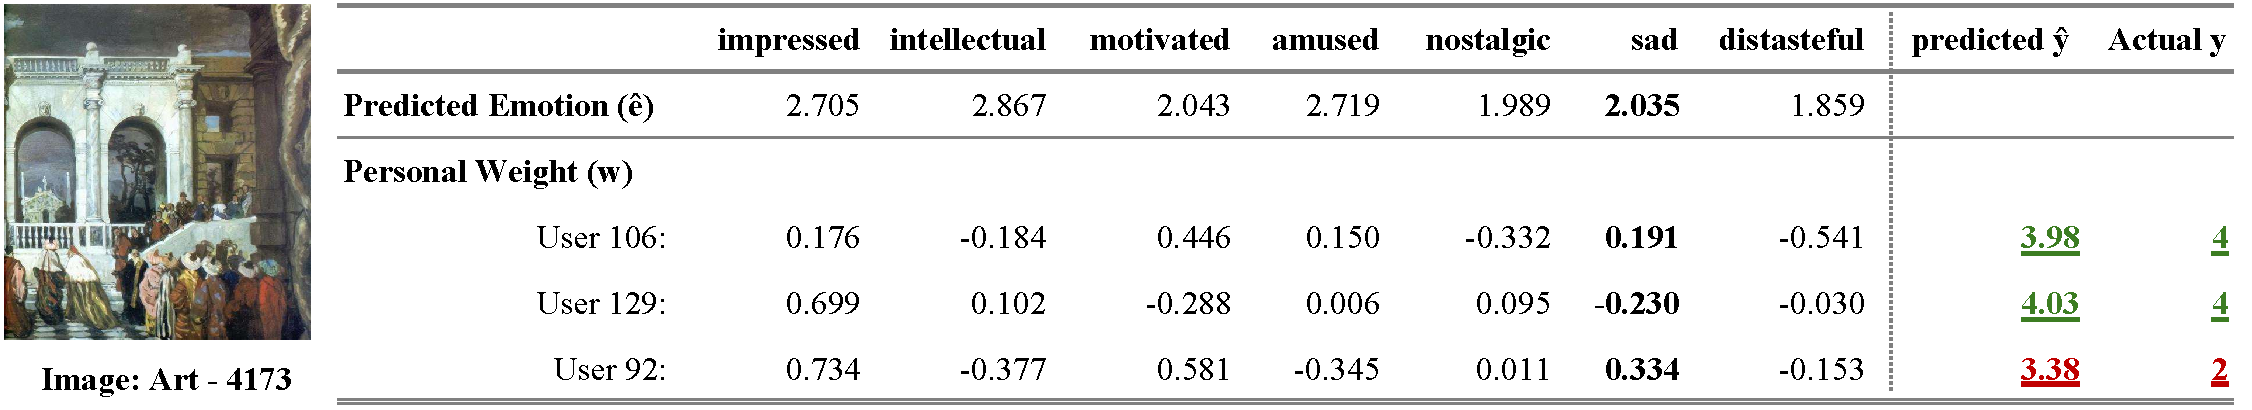
\includegraphics[width=\linewidth]{Table_Figure/fig_qualitative.pdf}
%     \caption{\textbf{Qualitative example of personal formulas and failure case.} 
%     For a shared artwork image (ID: 4173), we show the Stage-1 predicted emotion vector $\hat{\mathbf{e}}$, individual weight vectors $\mathbf{w}$, predicted rating $\hat{y}$, and actual rating $y$. 
%     \textbf{Selection criteria:} Users~106 and 129 were selected as a pair sitting at opposing ends of the Sad-weight distribution ($w_{\text{sad}} = +0.191$ vs.\ $-0.230$) with minimal prediction error on this image ($|y - \hat{y}| \le 0.03$). User~92 was selected on the same image as a failure case ($y = 2.0$, $\hat{y} = 3.38$)}
%     \label{fig:qualitative}
% \end{figure*}